\begin{frame}
    \frametitle{Physics of what we calculate}

    \begin{columns}
        \column{0.4\textwidth}
            \begin{wideitemize}
                \item Content of my Practical Training (Fachpraktikum)
                \item Hubbard Model Hamiltonian
                \item System under influence of external electric field
            \end{wideitemize}

        \column{0.5\textwidth}
            \makebox[\textwidth][c]{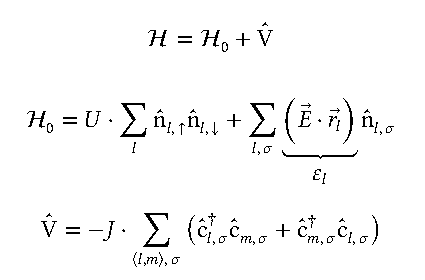
\includegraphics[width=\textwidth]{./main-content/physics/hamiltonian.pdf}}

    \end{columns}
\end{frame}

\begin{frame}
    \frametitle{Physics of what we calculate}

    \begin{columns}
        \column{0.4\textwidth}
            \begin{wideitemize}
                \item 2-dimensinal geometry
                \item Square lattice arrangement
                \item Computation for general size and field angle
            \end{wideitemize}
            
            \vspace{0.5cm}
            \begin{itemize}
                \item[Goal:]
                Approximate evaluation of time-evolution
            \end{itemize}

        \column{0.5\textwidth}
            \makebox[\textwidth][c]{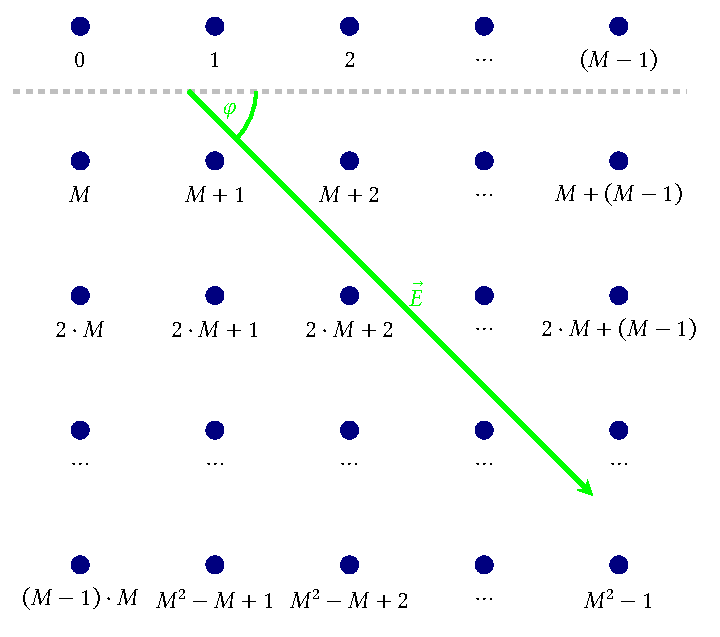
\includegraphics[width=.8\textwidth]{./main-content/physics/geometry.pdf}}
            
    \end{columns}
\end{frame}

\begin{frame}
    \frametitle{Physics of what we calculate}

    \begin{columns}
        \column{0.4\textwidth}
            \begin{wideitemize}
                \item Hard-Core Bosonic operators
                \begin{itemize}
                    \item (Would work analogously with Fermionic operators)
                \end{itemize}
                \item Two spin-degrees of freedom rewritten in alternate notation
            \end{wideitemize}

        \column{0.5\textwidth}
            \makebox[\textwidth][c]{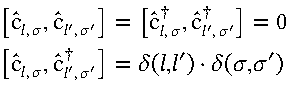
\includegraphics[page=1,width=.7\textwidth]{./main-content/physics/rewrite.pdf}}
            \makebox[\textwidth][c]{\includegraphics[page=2,width=.7\textwidth]{./main-content/physics/rewrite.pdf}}
            \makebox[\textwidth][c]{\includegraphics[page=3,width=.7\textwidth]{./main-content/physics/rewrite.pdf}}
            
    \end{columns}
\end{frame}